\documentclass[11pt,letterpaper]{article}

\usepackage{latexsym}
\usepackage{fancybox}
\usepackage{graphicx}
\usepackage{soul}
\usepackage{amssymb}
\usepackage{color}
\usepackage{ulem}
\usepackage{float}
\usepackage{xspace}
\usepackage{graphics}
%\usepackage{rotating}
\usepackage{setspace}
\usepackage{multirow}
\usepackage[abs]{overpic}
\usepackage{url}
\usepackage[font=scriptsize,labelfont=bf]{caption}
\usepackage{enumitem}
\usepackage{wrapfig}
\usepackage{tabu}
\usepackage{pgfgantt}

\usepackage{natbib}
\setlength{\bibsep}{0pt}
\citestyle{plain}

% Some fancy commenting
\definecolor{todo}{RGB}{200,0,0}
\newcommand{\comment}[2][todo]{{\color{#1}[[{\bf #2}]]}}

%\input{defs}
%\newcommand{\annrev}{ARA\&A}
\newcommand{\apj}{ApJ}%% Journal abbreviations
\newcommand{\apjs}{ApJS}
\newcommand{\apjl}{ApJL}
\newcommand{\aap}{A{\&}A}
\newcommand{\aaps}{A{\&}AS}
\newcommand{\mnras}{MNRAS}
\newcommand{\aj}{AJ}
\newcommand{\araa}{ARAA}
\newcommand{\pasp}{PASP}
\newcommand{\nat}{Nature}
\newcommand{\procspie}{Proc. of SPIE}

\let\la=\lesssim            % For Springer A&A compliance...
\let\ga=\gtrsim
\newcommand\sq{\mbox{\rlap{$\sqcap$}$\sqcup$}}%
\newcommand\arcdeg{\mbox{$^\circ$}}%
\newcommand\arcmin{\mbox{$^\prime$}}%
\newcommand\arcsec{\mbox{$^{\prime\prime}$}}%
\newcommand\fd{\mbox{$.\!\!^{\mathrm d}$}}%
\newcommand\fh{\mbox{$.\!\!^{\mathrm h}$}}%
\newcommand\fm{\mbox{$.\!\!^{\mathrm m}$}}%
\newcommand\fs{\mbox{$.\!\!^{\mathrm s}$}}%
\newcommand\fdg{\mbox{$.\!\!^\circ$}}%
\newcommand\farcm{\mbox{$.\mkern-4mu^\prime$}}%
\newcommand\farcs{\mbox{$.\!\!^{\prime\prime}$}}%
\newcommand\fp{\mbox{$.\!\!^{\scriptscriptstyle\mathrm p}$}}%
\newcommand\micron{\mbox{$\mu$m}}%

\makeatletter
\newcommand*{\rom}[1]{\expandafter\@slowromancap\romannumeral #1@}
\makeatother

\pretolerance=10000
\textwidth=7.25in
\textheight=9.9in
\voffset = -0.7in
\topmargin=0.0in
\headheight=-0.1in
\hoffset = -0.3in
\headsep=0.4in
\oddsidemargin=0in
\evensidemargin=0in
\parindent=1.2em
\parskip=0.1ex

\newcommand{\sqdeg}{\ensuremath{\mathrm{deg}^2}}
\newcommand{\sqarcmin}{\ensuremath{\mathrm{arcmin}^2}}
\newcommand{\nm}{\ensuremath{\mathrm{nm}}}
\newcommand{\ang}{\ensuremath{\mathrm{\AA}}}
\newcommand{\mpc}{\ensuremath{h^{-1}\,\mathrm{Mpc}}}
%\newcommand{\micron}{\ensuremath{\mu\mathrm{m}}}
\newcommand{\texp}{\ensuremath{t_\mathrm{exp}}}

\begin{document}

% Go for customized headings
\pagestyle{myheadings}
\markboth{\hfill \footnotesize 2018 Keck Instrumentation White Paper: FOBOS \hfill}{\hfill \footnotesize 2018 Keck Instrumentation White Paper: FOBOS \hfill}
\vspace*{-0.3in}
\noindent
%\doublespacing
\begin{centering}
\Large \textbf{The Keck Fiber-Optic Broadband Optical Spectrograph, FOBOS} \\
\end{centering}
\vspace{0.5em}
\noindent
\begin{centering} \small
%
K.~Bundy (UCO), K.~Westfall (UCO), K.-G.~Lee (IPMU/LBNL), N.~MacDonald
(UCO), D.~Schlegel (LBNL), R.~Kupke (UCO), T.~Miller (LBNL/SSL),
R.~M.~Rich (UCLA), C.~Rockosi (UCSC/UCO), J.~X.~Prochaska (UCSC/UCO),
C.~Poppet (UCB), K.~Zhang (LBNL)
%
\vskip 0.5em
\textit{8 June 2018} \\
\end{centering}

\noindent\begin{center}\mbox{\parbox{0.9\linewidth}{
%
The Fiber-Optic Broadband Optical Spectrograph (FOBOS) satisfies a top
priority for a highly sensitive and highly multiplexed Keck instrument
as identified in the Keck Strategic Plan.  In the past year, the FOBOS
team has completed a UCO-funded design of the microlens optics that deliver
high-throughput coupling of fibers to the Keck focal plane.  Meanwhile,
substantial synergies with the fiber-based version of TMT's Wide-Field
Optical Spectrograph (Fiber-WFOS) have retired sky-subtraction risks for
FOBOS, provided a head-start on designing other key components, and
identified exciting new options for added scientific capabilities.  Our
goal in this submission is to lay the groundwork for a conceptual design
phase (CDP) that would begin in 2019.  Doing so requires input from the
community on the following science-driven design questions: {\bf 1})
Should FOBOS adopt new WFOS-like spectrograph designs in order to push
UV sensitivity down to 310 nm? {\bf 2}) What is the optimal spectral
resolution or set of spectral resolutions for FOBOS? {\bf 3}) How
important is spatially-resolved spectroscopy to FOBOS science?  We
request \emph{\$50k} to work with the Keck community as well as our
FOBOS and Fiber-WFOS design teams to answer these questions. }
%
}\end{center}

\noindent{\Large\bf Motivation}

% UNCOMMENT THIS TO GET THE NO-INSET VERSION
%\begin{wrapfigure}{l}{0.4\textwidth}\small
%%
%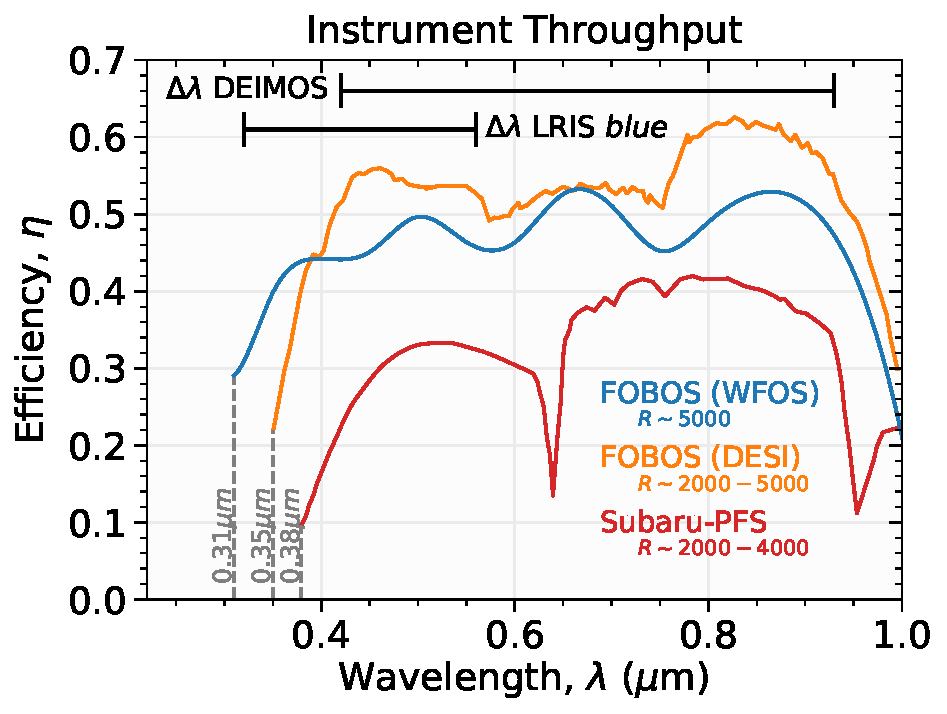
\includegraphics[width=0.4\textwidth]{./figs/throughput_comparison_noinset.pdf}
%%
%\caption{\label{fig:throughput} Expected instrument (fibers, coupling,
%spectrograph, and detector) performance for FOBOS, using either a WFOS
%or DESI spectrograph, compared to the Subaru-PFS spectrograph.
%%, including fiber transmission losses.
%The blue cutoff-wavelengths of each curve are annotated to emphasize the
%difference in blue response.  For reference, we show the spectral
%coverage, $\Delta\lambda$, for the 600/4000 grism for LRIS {\it blue}
%and the 1200G grating for DEIMOS are shown, defined by the region where
%the spectral efficiency is at least 10\% of the peak.  }
%%
%\end{wrapfigure}

\begin{wrapfigure}{l}{0.4\textwidth}\small
%
\includegraphics[width=0.4\textwidth]{./figs/throughput_comparison.pdf}
%
\caption{\label{fig:throughput} Expected instrument (fibers, coupling,
spectrograph, and detector) performance for FOBOS, using either a WFOS
or DESI spectrograph, compared to the Subaru-PFS spectrograph.
%, including fiber transmission losses.
The inset panel emphasizes FOBOS's blue sensitivity compared to PFS,
even when excluding the different telescope apertures.  For reference,
we show the spectral coverage, $\Delta\lambda$, for the 600/4000 grism
for LRIS {\it blue} and the 1200G grating for DEIMOS are shown, defined
by the region where the spectral efficiency is at least 10\% of the
peak.
%KG: Added that fiber losses are included Also shown is the ``total''
%Fiber-WFOS throughput (includes the microlens and fiber system).
} \end{wrapfigure}

\noindent {\bf Science Justification:} To stay competitive in the coming
era of deep, wide-field surveys (Gaia, LSST, WFIRST, and Euclid), the
2016 Keck Scientific Strategic Plan (SSP) lists {\bf sensitive, highly
multiplexed} spectroscopy as a top priority. 
%Keck's most highly multiplexed instrument, DEIMOS, currently has a
%multiplex of $\sim$140 slits compared to the 2400 fibers of the
%upcoming Subaru Prime Focus Spectrograph (PFS).  KG: We should also
%mention sensitivity immediately 
The SSP calls for an improved multiplex over a larger field-of-view than
currently available with DEIMOS ($\sim$140 over
16\arcmin$\times$4\arcmin), while also improving the blue coverage if
possible. 
%KG: I'm not sure we want to mention the PFS multiplex, since its
%unlikely that FOBOS would be able to achieve that
FOBOS can achieve these goals using a fiber-based system to improve
multiplex ($\sim$400--600) and sample Keck's full field-of-view, all
while simultaneously observing the entire optical wavelength range from
near-UV to near-IR at medium resolution.
%KG: Added a brief high-level summary of FOBOS. KBW: I edited this.
%There was a very similar sentence at the beginning of the PFS section.  
%I left this one here and removed that one.

Keck-community interest in FOBOS is substantial and broad, as evidenced
by the science presentations from participants at UCO-funded workshops
held over the past year.\footnote{See, e.g.,
\url{http://bccp.berkeley.edu/2018-multiplex-fiber/}}  FOBOS would be
the premier instrument for mapping IGM and CGM structure via
Lyman-$\alpha$ tomography at high redshift and over significant volumes.
It would spatially map Lyman-$\alpha$ nebula complexes across arcmin
scales, identifying regions of interest for KCWI followup.  It would
spearhead photo-$z$ training efforts at faint magnitudes necessary for
the success of wide cosmological imaging surveys (e.g., LSST).  It would
characterize the kinematics and populations of faint stellar systems
with high target densities in the Local Group.  And, when deploying
multiplexed IFUs, it will open new scientific areas including kinematic
weak lensing and GLAO-aided resolved spectroscopy of $z$$\sim$1
galaxies.  A single, over-sized fiber IFU at the field center would
provide instantaneous spectroscopic follow-up of targets of opportunity.

\noindent {\bf Demonstrating high sensitivity:} Keck's traditional
strength of {\bf faint-object} spectroscopy remains a high priority for
FOBOS.  Thankfully, recent advances in fiber-related technologies now
enable designs that can achieve \emph{both} high multiplex and high
sensitivity.  The combination of new fiber materials, short fiber runs
($\sim$10m), and improved grating technologies deliver total-instrument
throughput in the blue that are 85--95\% of what can be achieved by
modern slit spectrographs.  Such technical advances have motivated the
fiber-based instruments on both 8- and 30-meter telescopes, as well as
an intense study for a fiber-based design of TMT-WFOS (Fiber-WFOS).
Meanwhile, we have demonstrated that sky-subtraction systematics are
negligible with sky-nodding (Bundy et al.\ {\it in prep}), and a recent
21-hour MaNGA integration (Gu et al.\ 2018, ApJ, 859, 37) reached 0.2\%
background precision, the equivalent of a 22.8 AB source at $S/N = 5$ in
1 hour on Keck.
% Moreover, the FOBOS concept of siting the spectrographs on or near the
% Nasmyth deck allows a short fiber run ($<$10m) which reduces fiber
% throughput losses, especially in the blue.
%KG: Added sentence specifying short fibers.  KBW: I shortened this by
%adding a phrase above.

\noindent {\bf Uniqueness compared to Subaru-PFS:}
%FOBOS would provide a multiplex of $\sim$400-600 across the 
% unvignetted Keck focal plane, with simultaneous spectral coverage
%from the near-UV to the near-IR wavelengths at medium spectral
%resolution.
FOBOS differentiates itself
from Subaru PFS by optimizing for depth (not area/multiplex), providing
greater sensitivity over their common bandpass and far to the blue of 
the PFS's 0.38\micron\ limit (Figure
\ref{fig:throughput}),\footnote{PFS throughput data taken from
\url{http://pfs.ipmu.jp/research/parameters.html}} and enabling new
science with multiplexed integral-field-unit (IFU) spectroscopy.  If a
\textbf{ground-layer adaptive optics (GLAO)} system becomes feasible on
Keck, FOBOS will benefit from both the additional sensitivity gains and
improved spatial resolution, particularly for the IFUs.  \smallskip
%KG: Moved GLAO to here as a further differentiation from PFS

\noindent{\Large\bf Urgent Design Questions}

\noindent Our goal in the next phase of FOBOS development is to settle
fundamental design questions based on Keck community input in order to
prepare for a conceptual design phase.

% While FOBOS previously considered only the DESI spectrograph design
% heritage, alternative designs emerging from the TMT-WFOS team has
% opened up the parameter space that now needs to be considered:

%KG: Moved first mention of the fiber-WFOS design here to make it clear
%for the folllowing discussion. KBW: We're hurting for space.
%Fiber-WFOS is now mentioned well above and in the abstract  I removed
%the last sentence.

\noindent {\bf Spectral Range:}  A traditional strength of Keck has been
the {\bf blue sensitivity} of its instruments.  Although a redesign
could improve the DESI spectrograph's response below 0.36\micron, the
Fiber-WFOS spectrograph is explicitly designed to yield sensitivity at
even 0.31\micron. 
%KG: Modified to mention possibility of redesigning DESI blue limit.
%KBW: Edited this down.
However, Fiber-WFOS spectrographs will require more up-front design work
and may be more expensive, depending on the focal-plane format adopted.
There is also interest in pushing the red spectral limit into the
$J$-band to, e.g., observe H$\alpha$ and [O{\small \rom{2}}] emission at
$z$$\approx$1 and 2, respectively, and we plan to explore upgrade paths
for including a $J$-band channel in FOBOS.  The FOBOS work we propose
here will quantify these trades and compare them against community
science interests, e.g., within the context of Subaru PFS, so that a
baseline spectrograph design can be adopted.
%KG: Removed specific mention of fiber-WFOS regarding the NIR channel,
%since we'd also want to explore it for DESI

\begin{wrapfigure}{l}{0.4\textwidth}\small
\includegraphics[width=0.4\textwidth]{./figs/fobos_microlens.png}
\caption{\label{fig:microlens} The diagram of the FOBOS microlens design
used in our UCO-funded feasibility study.  The input $f$/15.2 Keck beam
is converted to an $f$/3.9 input to the fiber such that each fiber
subtends $0\farcs46$ on sky.} \end{wrapfigure}
%
\noindent{\bf Spectral Resolution:}  The FOBOS spectrographs will be
bench mounted and work under a fixed gravity vector, which benefits the
instrument stability.  However, we also expect the spectrographs will
have no moving parts, meaning the desired spectral resolution must be
chosen at the design stage following community input.  Both DESI and
Fiber-WFOS provide compelling options, delivering $R$$\sim$5000 at red
wavelengths for robust removal of the OH night-sky lines.  The WFOS team
is also exploring $R$$\sim$3500 designs that will be similarly
sufficient and meet the requirements of most galaxy science.  However,
some stellar-abundance work requires higher resolution.  For example,
detailed abundances of O, Mg, and r-process elements (e.g., Eu, La)
require $R$$\sim$15k in the 0.6--0.7\micron\ region.  We continue to
seek community feedback on the capabilities of our current sketch of an
$R$$\sim$15k spectrograph and its priority versus cost.  In general,
this and other purpose-built fiber-fed instruments could integrate
easily with FOBOS's focal plane system, opening up valuable upgrade
paths.

\noindent{\bf Spatial Sampling at the Focal Plane:}  Fibers at the FOBOS
focal plane can be deployed in a variety of ways that involve trades in
multiplex, target density, field-of-view, and 2D
spatial information from IFUs.  Several modes could be made available,
allowing users to select the mode appropriate for their science.

For a configuration demanding high multiplex, the spectrograph fiber
diameter and the angle it subtends on-sky is important.  For sufficient
aperture sizes with the relatively small DESI fibers, close-packed
7-fiber bundles coupled to a microlens array (Figure
\ref{fig:microlens}) are required.  However, a single WFOS spectrograph
with larger fibers could provide individual apertures of
$\sim$$1\arcsec$ with a multiplex of $\sim$650 at a similar cost as 4
DESI spectrographs with a multiplex of $\sim$400.  Unfortunately, a
single fiber, unlike the 7-fiber bundle, delivers no spatial
information.  A key question is how valuable are the 7-fiber bundles to,
e.g., kinematic weak lensing studies and/or PSF-characterization for
precise flux calibration?  

There is also substantial interest in deploying FOBOS fibers as 20--40
independently positioned IFUs for resolved spectroscopy.  This would
allow new science, including mapping nebular emission lines and outflow
signatures (e.g., [Mg {\small \rom{2}}]) of large numbers of galaxies
near $z$$\sim$1.   Moreover, a single IFU fixed at the center of the
field would allow for instantaneous target-of-opportunity follow-up.
We seek science-driven requirements than will help us plan and design
for these possible modes.  Given the significant gains for IFU science,
we will also work with the Keck GLAO team to study the feasibility of
wide-field correction and the instrument requirements (e.g., wave-front
sensors) needed for FOBOS to take advantage of GLAO.
%KG: Added sentence on GLAO
\smallskip

% requires thinking upfront about the focal plane layout (making space
% for wavefront sensors) and the optical design. We want to ensure that
% a modification to the microlens array foreoptics can provide adequate
% GLAO spatial sampling in this mode (e.g., 0.2 arcsec) without
% requiring changes to the spectrograph design.

\noindent{\Large\bf Proposed Work and Budget}

\noindent {\bf This Proposal:} We request \emph{\$50k} in funding from
W.~M.\ Keck Observatory (WMKO) to build toward a conceptual design phase
(CDP) to begin in 2019.  Our main goals, as motivated above, are to (1)
quantify and optimize the scientific and budgetary trades for the
instrument and (2) engage with the Keck community to build out a set of
well-motivated science and instrument requirements based on these trade
studies.  These activities will allow us to quickly converge on a
conceptual design for which we can construct a comprehensive budget to
present to funding agencies.
\medskip

\noindent We expect this requested amount from WMKO to be allocated as
follows:

{\bf 1) Spectrograph Design: \$25k}.  The scientific and budgetary
trades involved with the spectral resolution, spectral range, and system
efficiency will dominate our efforts in this phase.  This will involve
optical engineering of the spectrographs along multiple avenues,
including the number of spectral channels and the spectral resolution
necessary for sky subtraction and specific science goals.

{\bf 2) Scientific Trades from Spatial Sampling Options: \$15k}.  The
flexibility of the focal plane to multiple reformatting possibilities
will have to be constrained by a phased development of the instrument.
A study is required to develop the strategy that leads to the most
timely science being produced by the instrument, particularly given the
trades between multiplex and spatial sampling and resolution.

{\bf 3) Scientifically Motivated Instrument Requirements: \$10k}.  Key
to the success of FOBOS is to engage the community in the design trades
discussed above.  These trade studies will naturally lead to a set of
development options and hard choices in terms of FOBOS's capabilities.
We will build science teams --- via both one-on-one interaction in
institution visits and topical workshops --- that will help guide an
instrument requirements document needed to focus the future funding and
development efforts for FOBOS.
\medskip

\begin{wrapfigure}{l}{0.45\textwidth}\small
%
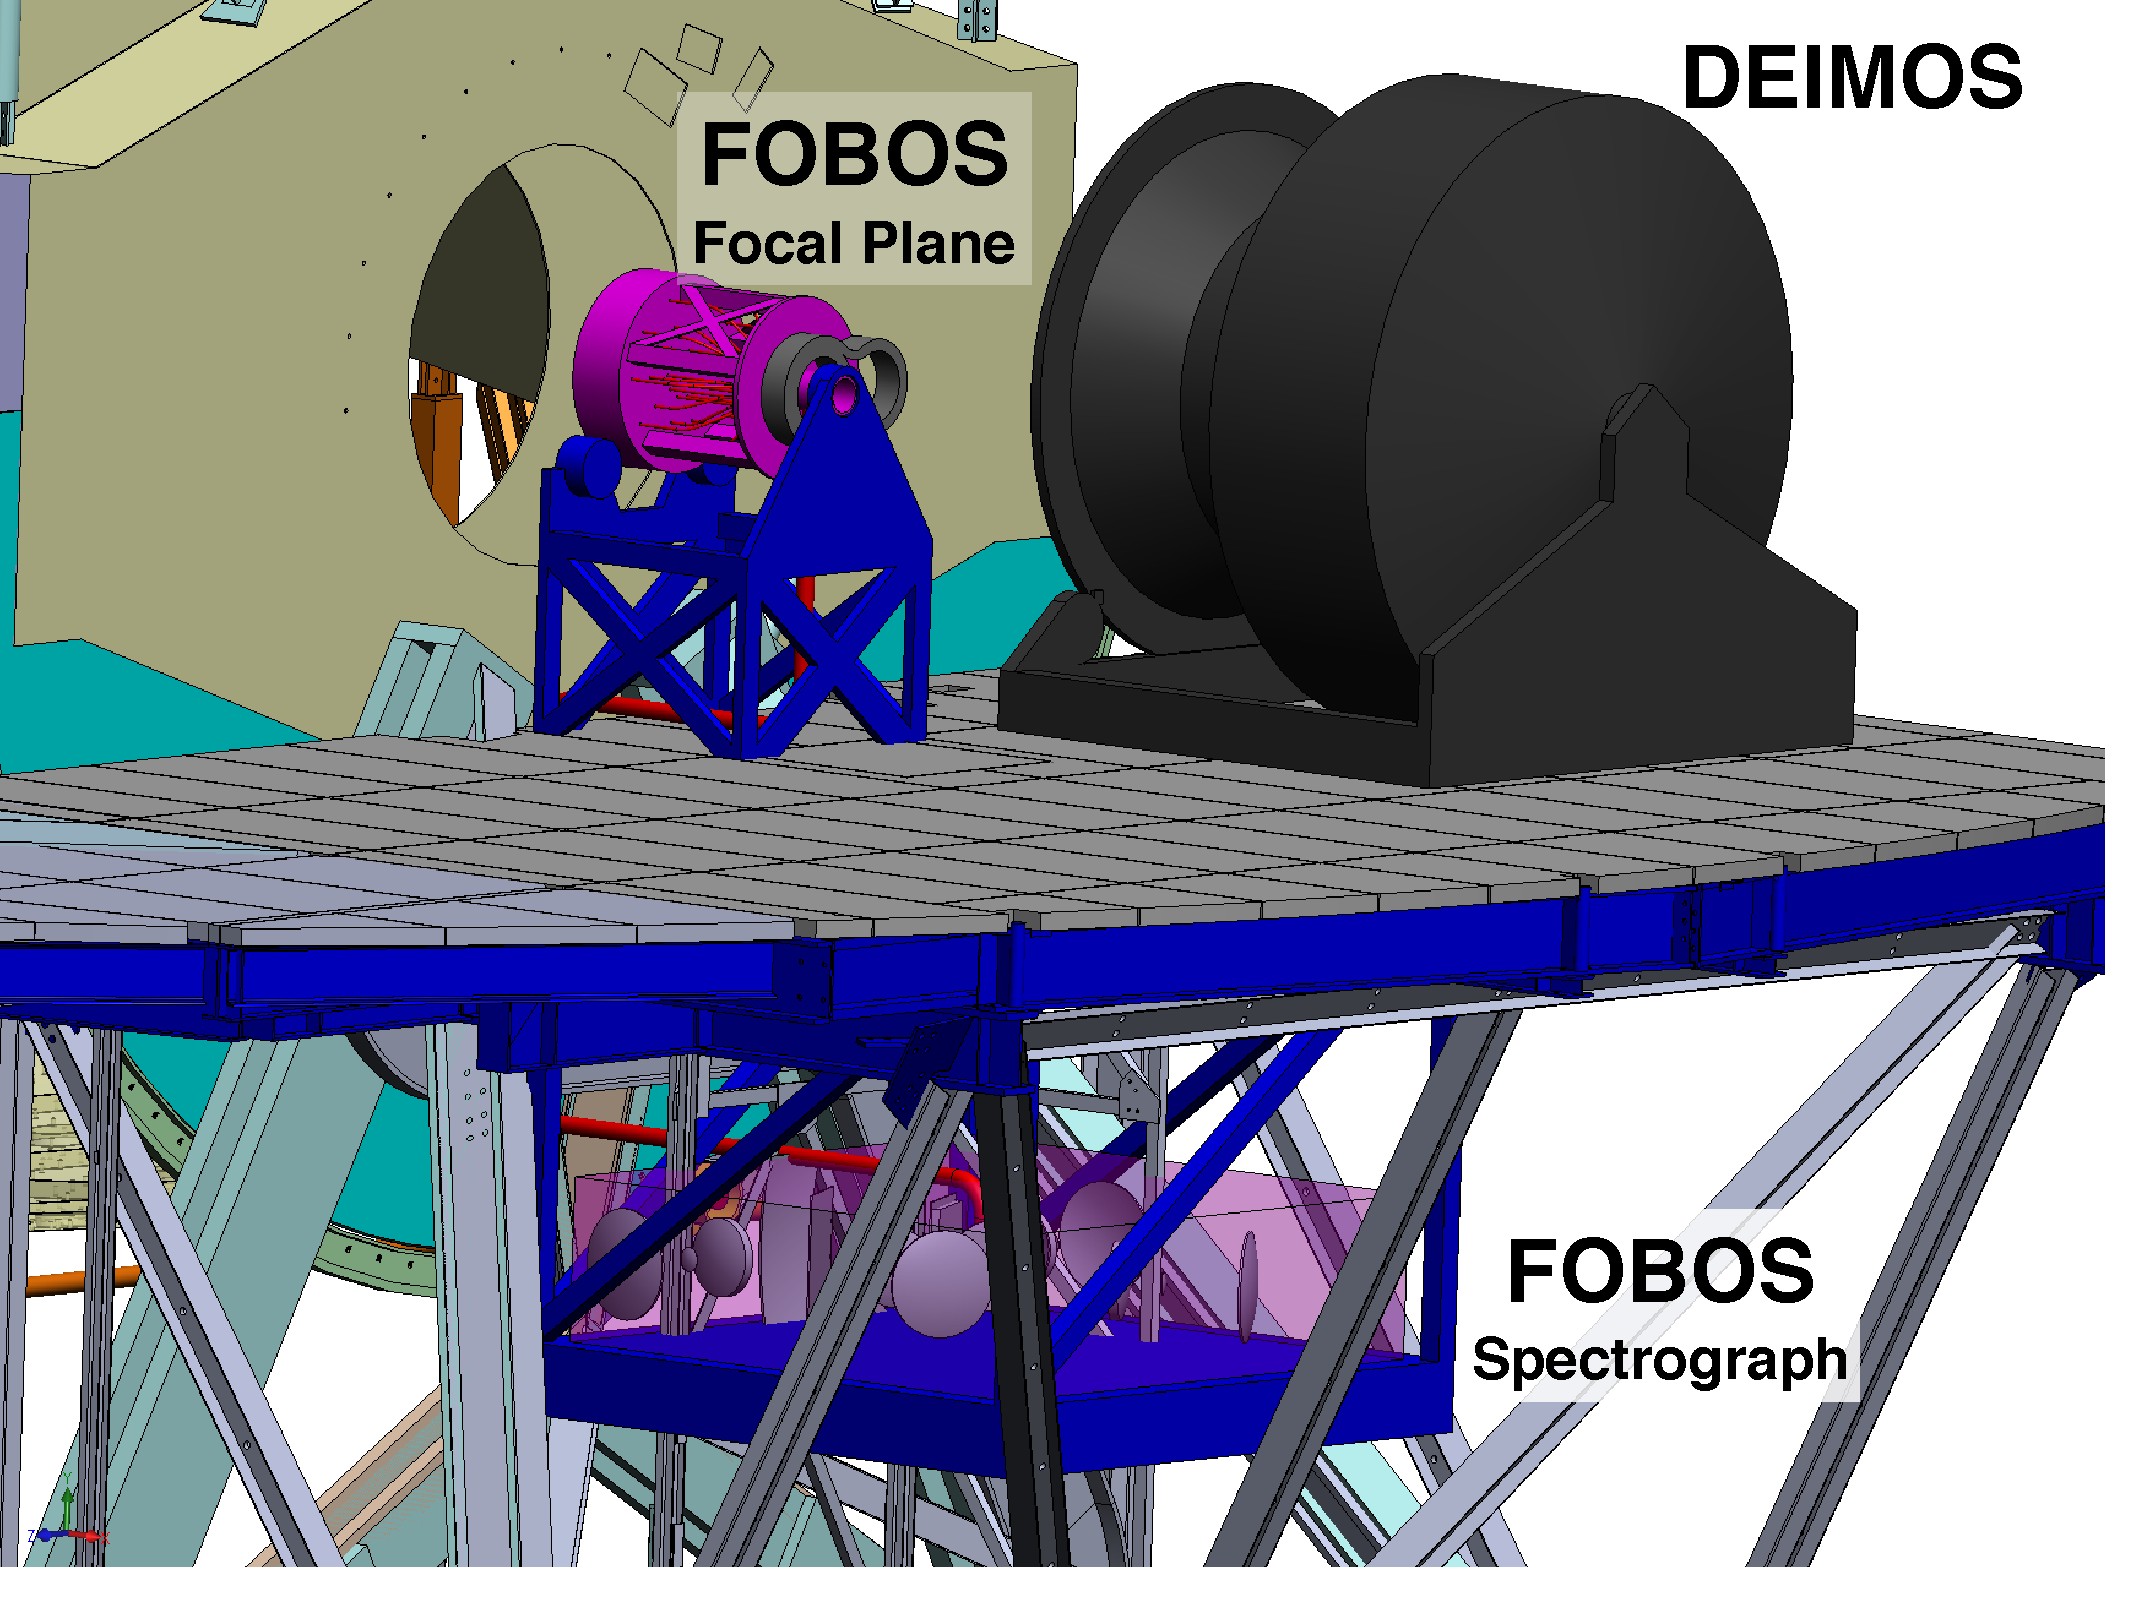
\includegraphics[width=0.45\textwidth]{./figs/FOBOSatKeck.pdf}
%
\caption{\label{fig:atkeck} A schematic diagram of FOBOS on Keck-2.  The
FOBOS focal-plane system, normally stowed in front of NIRSPEC, is shown
at the Nasmyth port next to the parked DEIMOS spectrograph.  Here, the
focal-plane feeds the bench-mounted Fiber-WFOS spectrograph housed below
the platform.}
% KG: Added that stowage position in front of NIRSPEC 
\end{wrapfigure}

% Our requested funding of {\bf \comment{\$50k}} will allow us to build
% a conceptual design of FOBOS by exploring the key design trades
% discussed above, as it relates to the scientific capabilities of the
% instrument.  These funds are broken down as follows: %
% \begin{enumerate}
% 
% \item {\bf Multi-channel Spectrograph: \$20k} -- 3 months at 0.3 FTE.
% The key spectrograph design trades are the blue sensitivity and the
% spectral resolution.  Our trade study will draw from both the DESI and
% fiber-WFOS designs, but maximize the performance of FOBOS for Keck.
% For example, substantial effort at UCO by the WFOS team has led to a
% 4-channel, fiber-fed spectrograph with excellent blue throughput
% (end-to-end performance, including a 10m fiber run, is $\sim$30\% at
% 0.31\micron).  Only modest alterations would be needed to adapt it for
% Keck given the microlens coupling to the fiber feed.  However, as also
% being pursued for TMT, we may want to decrease the resolution in the
% blue ($R$$\sim$2000; although the fiber-WFOS-like requirement of
% $R$$\sim$5000 may be more appropriate for stellar-abundance science)
% such that we remove the reddest channel from that design.
% 
% Modest work will include design changes that accommodate multiple
% pseudoslits, as needed for multiple (e.g., unresolved vs. resolved)
% focal-plane formats.  Finally, design work will also include allowing
% for a $J$-band channel, most likely as an upgrade path dependent on
% the maturation of Ge CCD detector technology.
% 
% \item {\bf Focal-Plane System: \$15k} -- 2 months at 0.3 FTE.  The key
% design trades for the focal-plane system are the positioning mechanism
% and the flexibility to multiple formats.  There is significant
% interest in both single-spectrum and resolved, integral-field
% spectroscopy with FOBOS; the latter is particularly interesting for
% taking full advantage of GLAO.  There are a number of ways that we can
% accommodate multiple formats in the FOBOS focal plane; however, some
% of these come with trades that could limit 
% 
% both small-scale integral collectors and larger-format integral-field
% units for resolved spectroscopy, particularly for taking advantage of
% GLAO performance improvements.  Designs exist for how fiber-WFOS would
% take advantage of 
% 
% 
% a positioning system suitable to the largest number of scientific
% programs, that provides a maximally configurable positioning system,
% and, if possible, can easily accommodate multiple fiber inputs that
% provide additional formats via a slit exchanger or additional fiber
% feeds from subsequent facility instruments.  % \item {\bf Community
% Engagement: \$15k} -- \$10k in travel, \$5k for workshops.  Key to the
% success of FOBOS is to engage the community in the design trades
% discussed abbove.  % \end{enumerate}


\noindent {\bf Update on Previous Work and Development:} We have
recently completed a UCO-funded feasibility study of the microlens
system to couple the Keck focal plane with FOBOS fibers; a full report
is available at \url{http://bit.ly/FobosML_May2018}.  In short, we find
no technical issues that prove limiting to the FOBOS concept, although
pistoning robotic positioners might be required to address astigmatism
at the edges of the Keck focal plane.

Also, we have recently visited WMKO and identified several options for
installing FOBOS on Keck-2 without disturbing existing instruments.  The
focal plane system can be slotted into the Nasmyth port using a cart
similar to other instruments, whereas the spectrograph(s) can be mounted
under the Nasmyth deck as shown in Figure \ref{fig:atkeck}.
%KG: Specified that it's Keck-2 being discussed.

Compared to previous years, there are even more reasons to
pursue synergies with the build-up of fiber-based facilities at UCO and
the ongoing development of TMT-WFOS.  Although TMT-WFOS has not yet
decided between a slit-based or fiber-based design, FOBOS can benefit
from the direct involvement of the WFOS design team.  If the slit-based
design is selected, the already completed Fiber-WFOS design work
immediately benefits FOBOS by providing a highly efficient alternative
spectrograph design that specifically provides blue sensitivity.  One could think of
this as ``matching funds'' for UCO's investment in FOBOS.  Even more
synergies are, of course, expected if Fiber-WFOS is selected by TMT.  In fact, we estimate that {\it each} project
would save roughly \$3M in shared development costs.  This expected synergy has
led to greater involvement in FOBOS from the TMT-WFOS team members.
In collaboration with the fiber-based instrumentation expertise at LBNL,
there is a clear path for development of both WFOS and FOBOS to be led by our UCO-based team. \medskip
%KG: Mentioned LBL involvement

% \begin{table}[h!]
% \centering
% \footnotesize
% \caption{Instrument Comparison}
% \label{tab:comparison} 
% \begin{tabular}{l | c | c | c | c}
%  & DEIMOS & PFS & FOBOS & FOBOS$+$ \\
% \hline
% Spectral Range (\micron) & 0.41--1.06 & 0.38--1.26 & 0.36--0.98 & 0.31--1.4 \\
% Multiplex  & 130 & 2400 & 400 & 800 \\
% Target Density (arcmin$^2$) & 1.7 & 0.6 & 2.5 & 5.0 \\
% Resolution ($R$) & 3000--6000 & 2300--5000 & 2000--5000 & 2000--5000 \\
% Survey Speed & 0.1 & 1.0 & 0.5 & 2.0 \\
% IFUs & no & no & 20 & 40 \\
% GLAO & no & no & yes & yes
% \end{tabular}
% \end{table}

{\small
%
\noindent{\it Acknowledgements:}  We would like to acknowledge, in
particular, the support of Claire Max, Jean Brodie, and Marc Kassis in
discussions of this white paper and FOBOS in general.  Their input has
been critical.  We would also like to thank all the attendees of the
FOBOS workshops who have helped us think through the design trades and
desirable capabilities of a fiber-based spectrograph at Keck, many of
which helped shape this white paper.
%
}

%{
%\footnotesize
%\bibliographystyle{apj}
%\bibliography{ref}
%}

%\noindent\begin{center}\mbox{\parbox{1.0\linewidth}{
%\twocolumn
%\footnotesize
%\bibliographystyle{apj}
%\bibliography{ref}
%}}\end{center}

\end{document}


% \noindent {\bf Sensitivity:} Of critical importance to the FOBOS design
% is to leverage the development and characterization of fiber-based
% spectrographs over the past 20 years, to optimize the system for depth
% and take full advantage of Keck's aperture and unvignetted
% field-of-view.  Indeed, in response to past submissions, the Keck
% Scientific Steering Committee (SSC) has expressed valid concerns about
% the depths to which FOBOS can maintain Poisson-limited signal-to-noise
% (S/N) growth as a function of exposure time; sub-Poisson performance has
% been demonstrated for numerous instruments \citep{2010MNRAS.408.2495S,
% 2013Msngr.151...10Y, 2016AJ....152...83L}.  However, as a result of some
% of our own work using OzDES \citep{2015MNRAS.452.3047Y} data and a very
% detailed analysis (Bundy et al., {\it in prep})\footnote{
% %
% Draft available upon request.\comment{check with Kevin}
% %
% } of SDSS-IV/MaNGA \citep{2015ApJ...798....7B} and VLT-GIRAFFE data, we
% are confident that any associated risk can be mitigated by a combination
% of hardware and software design.  A prediction based on the
% SDSS-IV/MaNGA data demonstrates an effective loss of, at most, 10\% in
% $g$-band exposure time for a 16-hour integration \comment{for TMT,
% translate to Keck, check with Kevin}.  This is an exceptional result
% given that the SDSS telescope \citep{2006AJ....131.2332G} and BOSS
% spectrographs \citep{2013AJ....146...32S} were not designed with such
% long integrations in mind \citep[cf.,][]{2017arXiv170907003G}.

% The primary hardware considerations are (1) a fast, telecentric fiber
% input beam to limit FRD, (2) a combined microlens and spectrograph
% design that accommodates the expected FRD for the fiber run based on
% preliminary lab testing, (3) sufficient scrambling of the near- and
% far-field illumination patterns to maximize the stability of the
% instrumental response at both low (broad-band throughput) and high
% frequencies (line-spread function, LSF), and (4) a combined focal-plane,
% pseudo-slit, and detector design that can accommodate multiple
% sky-subtraction strategies \citep{2001PASP..113..197G,
% 2010MNRAS.408.2495S, 2013Msngr.151...10Y}.  In fact, pioneering research
% in terms of instrument stability is currently being led by the
% planet-finding community \citep[e.g.,][]{2018ApJ...853..181P}, where
% their performance far exceeds our needs for FOBOS \comment{check this}.
% \comment{I'd also like a comment here about how other instruments
% (DESI?) have benefited from these principles in their design.}  Software
% considerations include appropriate control software and reduction
% techniques \citep[][Bundy et al., {\it in prep}]{2005ApJS..156..311B,
% 2010PASP..122..248B, 2013Msngr.151...10Y, 2016AJ....152...83L,
% 2018ApJ...858L..16W} that accommodate the sky-subtraction requirements
% of different programs.

% \noindent{\bf Facility benefits from FOBOS development}:
% %
% \begin{itemize}
% %
% \item detailed characterization of the optical performance and
% focal-plane characteristics of Keck (needed for microlens / spectrograph
% optimization?)
% %
% \item provides an ADC that can be used for other instruments (KPF)
% %
% \item provides a focal-plane system that can be designed to accommodate
% fiber feeds to multiple instruments (high-resolution spectrograph)
% %
% \item can be designed to take full advantage of GLAO upgrade
% %
% \end{itemize}

%\begin{figure}[ht]
%\includegraphics[width=0.35\textwidth]{fobos_microlens.png}
%\caption{\label{fig:microlens} The schematic diagram of the FOBOS
%microlens design.  The input $f$/15.2 Keck beam is converted to an
%$f$/3.9 input to the fiber such that each fiber subtends $0\farcs46$ on
%sky.  } \end{figure}
%
%\begin{figure}[ht]
%\includegraphics[width=0.35\textwidth]{throughput_comparison.pdf}
%\caption{\label{fig:throughput} Throughput comparison between
%Fiber-WFOS, DESI, and PFS.\footnote{Taken from the table at
%\url{http://pfs.ipmu.jp/research/parameters.html}}  Most data represent
%the expected performance of the spectrograph and detector system only;
%however, a ``total'' system performance for Fiber-WFOS is also shown,
%which includes the microlens and fiber system (dotted blue).  }
%\end{figure}
%
%\begin{figure}[ht]
%\includegraphics[width=0.35\textwidth]{FOBOS_01.pdf}
%\caption{\label{fig:atkeck} A schematic diagram of FOBOS at Keck.  The
%focal-plane system occupies a rather small footprint on the Nasmyth
%deck.  The bench-mounted Fiber-WFOS spectrograph is housed below the
%deck.}
%\end{figure}

%\begin{wrapfigure}{l}{0.35\textwidth}\footnotesize
%\includegraphics[width=0.35\textwidth]{fobos_microlens.png}
%\caption{\label{fig:microlens} The schematic diagram of the FOBOS
%microlens design.  The input $f$/15.2 Keck beam is converted to an
%$f$/3.9 input to the fiber such that each fiber subtends $0\farcs46$ on
%sky.  } \end{wrapfigure}
%
%\clearpage
%
%\begin{wrapfigure}{l}{0.35\textwidth}\footnotesize
%\includegraphics[width=0.35\textwidth]{throughput_comparison.pdf}
%\caption{\label{fig:throughput} Throughput comparison between
%Fiber-WFOS, DESI, and PFS.\footnote{Taken from the table at
%\url{http://pfs.ipmu.jp/research/parameters.html}}  Most data represent
%the expected performance of the spectrograph and detector system only;
%however, a ``total'' system performance for Fiber-WFOS is also shown,
%which includes the microlens and fiber system (dotted blue).  }
%\end{wrapfigure}
%
%\clearpage
%
%\begin{wrapfigure}{l}{0.35\textwidth}\footnotesize
%\includegraphics[width=0.35\textwidth]{FOBOS_01.pdf}
%\caption{\label{fig:atkeck} A schematic diagram of FOBOS at Keck.  The
%focal-plane system occupies a rather small footprint on the Nasmyth
%deck.  The bench-mounted Fiber-WFOS spectrograph is housed below the
%deck.} \end{wrapfigure}

% FOBOS as a concept continues to build on the science cases drawn from
% the UC community, as summarized \comment{below}.  These cases range
% from those that require $R$$\sim$15000 very high spectral resolution


%Past design work:
% - Microlens foreoptics to feed the fibers with a fast beam to minimize
%   focal-ratio degredation.
%
%Design work for this phase:
% - Spectral range (Reni, LBL?):
%    - Extension of the blue spectral coverage.  What is the blue
%      response of the Keck telescope?  How far can we push the DESI
%      design to take full advantage of this?  What would be our minimum
%      fiber run, and how does this affect our design choice for the blue
%      spectral range.
%    - Inclusion of a red arm that includes spectral coverage to
%      $\sim$1.3 micron.  Can we take advantage of upcoming advances in
%      detector technology, specifically Ge CCDs that are substantially
%      less expensive than PFS's detectors (need specific detector name)?
% - Spectral resolution (Reni, LBL?):
%
% - Focal plane:
%    - Continue development of the microlens technology to optimally feed
%      the instrument fibers with a fast, telecentric beam.  The
%      microlenses will both feed the fiber with a faster beam and
%      increase the on-sky aperture to more appropriately sample the Keck
%      PSF, with or without GLAO correction.
%    - 
%
% - ADC
%      
%      including a
%      detailed characterization of the Keck focal plane to 
%
% - Top-of-telescope throughput analysis for detailed science trade
%   studies.
